\documentclass[aspectratio=169,12pt,t]{beamer}
\usepackage{graphicx}
\setbeameroption{hide notes}
\setbeamertemplate{note page}[plain]
\usepackage{listings}

% header.tex: boring LaTeX/Beamer details + macros

% get rid of junk
\usetheme{default}
\beamertemplatenavigationsymbolsempty
\hypersetup{pdfpagemode=UseNone} % don't show bookmarks on initial view


% font
\usepackage{fontspec}
\setsansfont
  [ ExternalLocation = ../fonts/ ,
    UprightFont = *-regular ,
    BoldFont = *-bold ,
    ItalicFont = *-italic ,
    BoldItalicFont = *-bolditalic ]{texgyreheros}
\setbeamerfont{note page}{family*=pplx,size=\footnotesize} % Palatino for notes
% "TeX Gyre Heros can be used as a replacement for Helvetica"
% I've placed them in fonts/; alternatively you can install them
% permanently on your system as follows:
%     Download http://www.gust.org.pl/projects/e-foundry/tex-gyre/heros/qhv2.004otf.zip
%     In Unix, unzip it into ~/.fonts
%     In Mac, unzip it, double-click the .otf files, and install using "FontBook"

% named colors
\definecolor{offwhite}{RGB}{255,250,240}
\definecolor{gray}{RGB}{155,155,155}
\definecolor{purple}{RGB}{177,13,201}
\definecolor{green}{RGB}{46,204,64}

\definecolor{background}{RGB}{255,255,255}
\definecolor{foreground}{RGB}{24,24,24}
\definecolor{title}{RGB}{27,94,134}
\definecolor{subtitle}{RGB}{22,175,124}
\definecolor{hilit}{RGB}{122,0,128}
\definecolor{vhilit}{RGB}{255,0,128}
\definecolor{codehilit}{RGB}{255,0,128}
\definecolor{lolit}{RGB}{95,95,95}
\definecolor{myyellow}{rgb}{1,1,0.7}
\definecolor{nhilit}{RGB}{128,0,128}  % hilit color in notes
\definecolor{nvhilit}{RGB}{255,0,128} % vhilit for notes

\newcommand{\hilit}{\color{hilit}}
\newcommand{\vhilit}{\color{vhilit}}
\newcommand{\nhilit}{\color{nhilit}}
\newcommand{\nvhilit}{\color{nvhilit}}
\newcommand{\lolit}{\color{lolit}}

% use those colors
\setbeamercolor{titlelike}{fg=title}
\setbeamercolor{subtitle}{fg=subtitle}
\setbeamercolor{institute}{fg=lolit}
\setbeamercolor{normal text}{fg=foreground,bg=background}
\setbeamercolor{item}{fg=foreground} % color of bullets
\setbeamercolor{subitem}{fg=lolit}
\setbeamercolor{itemize/enumerate subbody}{fg=lolit}
\setbeamertemplate{itemize subitem}{{\textendash}}
\setbeamerfont{itemize/enumerate subbody}{size=\footnotesize}
\setbeamerfont{itemize/enumerate subitem}{size=\footnotesize}

% page number
\setbeamertemplate{footline}{%
    \raisebox{5pt}{\makebox[\paperwidth]{\hfill\makebox[20pt]{\lolit
          \scriptsize\insertframenumber}}}\hspace*{5pt}}

% add a bit of space at the top of the notes page
\addtobeamertemplate{note page}{\setlength{\parskip}{12pt}}

% default link color
\hypersetup{colorlinks, urlcolor={hilit}}

\lstset{language=bash,
        basicstyle=\ttfamily\scriptsize,
        frame=single,
        commentstyle=,
        backgroundcolor=\color{offwhite},
        showspaces=false,
        showstringspaces=false
        }


% a few macros
\newcommand{\bi}{\begin{itemize}}
\newcommand{\bbi}{\vspace{24pt} \begin{itemize} \itemsep8pt}
\newcommand{\ei}{\end{itemize}}
\newcommand{\be}{\begin{enumerate}}
\newcommand{\bbe}{\vspace{24pt} \begin{enumerate} \itemsep8pt}
\newcommand{\ee}{\end{enumerate}}
\newcommand{\ig}{\includegraphics}
\newcommand{\subt}[1]{{\footnotesize \color{subtitle} {#1}}}
\newcommand{\ttsm}{\tt \small}
\newcommand{\ttfn}{\tt \footnotesize}
\newcommand{\figh}[2]{\centerline{\includegraphics[height=#2\textheight]{#1}}}
\newcommand{\figw}[2]{\centerline{\includegraphics[width=#2\textwidth]{#1}}}


%%%%%%%%%%%%%%%%%%%%%%%%%%%%%%%%%%%%%%%%%%%%%%%%%%%%%%%%%%%%%%%%%%%%%%
% end of header
%%%%%%%%%%%%%%%%%%%%%%%%%%%%%%%%%%%%%%%%%%%%%%%%%%%%%%%%%%%%%%%%%%%%%%

% title info
\title{Computer simulations}
\subtitle{The genomes of recombinant inbred lines}
\author{\href{https://kbroman.org}{Karl Broman}}
\institute{Biostatistics \& Medical Informatics \\ Univ.\ Wisconsin{\textendash}Madison}
\date{\href{https://kbroman.org}{\tt \scriptsize \color{foreground} kbroman.org}
\\[-4pt]
\href{https://github.com/kbroman}{\tt \scriptsize \color{foreground} github.com/kbroman}
\\[-4pt]
\href{https://twitter.com/kwbroman}{\tt \scriptsize \color{foreground} @kwbroman}
}


\begin{document}

% title slide
{
\setbeamertemplate{footline}{} % no page number here
\frame{
  \titlepage

  \note{}

} }



\begin{frame}[c]{}

\vspace*{-1mm} \hspace*{-2mm}
\figw{Figs/inbredmice.jpg}{1.2}

\end{frame}




\begin{frame}{}

\vspace*{18mm}

\centerline{
\begin{minipage}[t]{50mm}
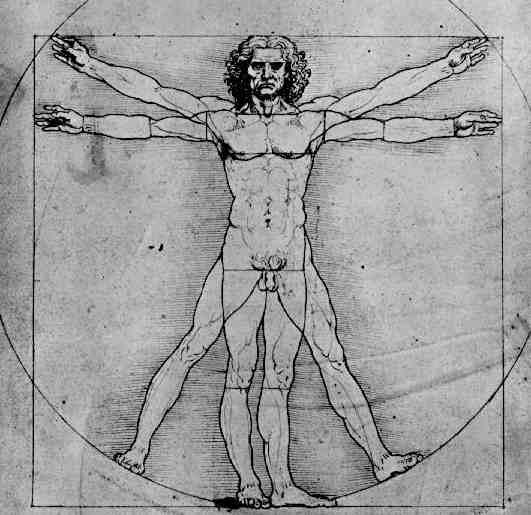
\includegraphics[height=50mm]{Figs/da-vinci-man.jpg}
\end{minipage}
\hspace{15mm}
\begin{minipage}[t]{50mm}
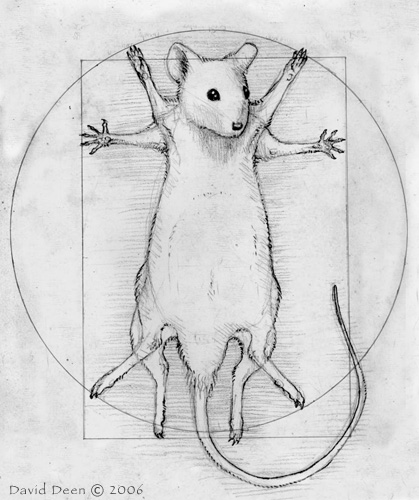
\includegraphics[height=50mm]{Figs/vitruvian_mouse.jpg}
\hspace{5mm}
\href{http://daviddeen.com}{\scriptsize \lolit \tt daviddeen.com}
\end{minipage}
}
\end{frame}





\begin{frame}[c]{Intercross}
\figw{Figs/intercross.pdf}{1.0}
\end{frame}





\begin{frame}[c]{QTL mapping}

\vspace{5mm}
\figw{Figs/lodcurve_insulin_with_effects.pdf}{0.96}
\end{frame}


\begin{frame}[c]{Congenic line/NIL}

\figw{Figs/congenic.pdf}{1.0}

\end{frame}




\begin{frame}[c]{Advanced intercross lines}

  \figw{Figs/ail.pdf}{1.0}

\end{frame}


\begin{frame}[c]{Recombinant inbred lines}

  \only<1>{\figw{Figs/rilines.pdf}{1.0}}
  \only<2>{\figw{Figs/riself.pdf}{1.0}}

\end{frame}


\begin{frame}[c]{Collaborative Cross}

  \figw{Figs/ri8.pdf}{1.0}

\end{frame}


\begin{frame}[c]{MAGIC}

  \figw{Figs/ri8self.pdf}{1.0}

\end{frame}



\begin{frame}[c]{Heterogeneous stock}

  \vspace{2mm}

  \figh{Figs/hs.pdf}{0.9}

\end{frame}


\begin{frame}[c]{Collaborative Cross}

  \figw{Figs/ri8.pdf}{1.0}

\end{frame}


\begin{frame}[c]{CC genome}

  \only<1>{\figw{Figs/ri8genome1.pdf}{1.0}}
  \only<2>{\figw{Figs/ri8genome2.pdf}{1.0}}
  \only<3>{\figw{Figs/ri8genome3.pdf}{1.0}}
  \only<4>{\figw{Figs/ri8genome4.pdf}{1.0}}
  \only<5>{\figw{Figs/ri8genome5.pdf}{1.0}}

\end{frame}


\begin{frame}[c]{Recombination fraction}
  \figw{Figs/basic_genetics.pdf}{1.0}
\end{frame}


\begin{frame}[c]{Simulation results}
  \figw{Figs/rf_by_sim.pdf}{1.0}
\end{frame}


\begin{frame}[c]{Haldane \& Waddington 1931}

  \figw{Figs/haldane_title.pdf}{0.9}

\end{frame}


\begin{frame}[c]{Result for selfing}

  \figw{Figs/haldane_selfing.png}{0.9}

\end{frame}


\begin{frame}[c]{Result for sib-mating}

  \only<1>{\figw{Figs/haldane_sibmating3.png}{0.9}}
  \only<2>{\figw{Figs/haldane_sibmating4.png}{0.9}}

\end{frame}


\begin{frame}[c]{Simulation results}
  \figw{Figs/rf_by_sim_genformula.pdf}{1.0}
\end{frame}



\begin{frame}[fragile]{Non-linear regression}

\vspace{5mm}

{
\verb|    out <- nls(| {\tt \vhilit R \verb|~| a*r/(1 + b*r)}\verb|,| \\
\verb|               data = data.frame(r=r, R=R),| \\
\verb|               start = list(a=4, b=6))| \\
\verb|    summary(out)|
}

\end{frame}


\begin{frame}[fragile]{Non-linear regression}
\addtocounter{framenumber}{-1}

\vspace{5mm}

\verb|    out <- nls(| {\tt \vhilit R \verb|~| a*r/(1 + b*r)}\verb|,| \\
\verb|               data = data.frame(r=r, R=R),| \\
\verb|               start = list(a=4, b=6))| \\
\verb|    summary(out)|

\vspace{8mm}

{\hilit
\verb|                          | \\
\verb|      Estimate  Std. Error| \\
\verb|    a    7.016       0.011| \\
\verb|    b    6.023       0.016|
}

\end{frame}


\begin{frame}[fragile]{Non-linear regression}
\addtocounter{framenumber}{-1}

\vspace{5mm}

\verb|    out <- nls(| {\tt \vhilit R \verb|~| a*r/(1 + b*r)}\verb|,| \\
\verb|               data = data.frame(r=r, R=R),| \\
\verb|               start = list(a=4, b=6))| \\
\verb|    summary(out)|

\vspace{8mm}

{\hilit
\verb|                                       More data      | \\
\verb|      Estimate  Std. Error        Estimate  Std. Error| \\
\verb|    a    7.016       0.011      a    7.003       0.008| \\
\verb|    b    6.023       0.016      b    6.005       0.012|
}

\end{frame}


\begin{frame}[c]{Simulation results}
  \figw{Figs/rf_by_sim_moredata.pdf}{1.0}
\end{frame}


\begin{frame}[c]{Markov chain}

\bbi
\item Sequence of random variables $\mathsf{\{X_0, X_1, X_2, \dots\}}$
  satisfying

\vspace{2mm}

\centerline{\hilit $\mathsf{Pr(X_{n+1} \ | \ X_0,
X_1, \dots, X_n) = Pr(X_{n+1} \ | \ X_n)}$}

\item Transition probabilities {\hilit $\mathsf{P_{ij} =
  Pr(X_{n+1} = j \ | \ X_n = i)}$}

\item Here, $\mathsf{X_n}$ = ``parental type'' at generation n.

\item We are interested in {\vhilit absorption probabilities}

\vspace{2mm}

\centerline{\hilit $\pi_j = \mathsf{Pr(X_n \rightarrow j \ | \ X_0)}$}
\ei

\end{frame}



\begin{frame}[c]{Absorption probabilities}

  \bbi

  \item[] Consider the case of {\vhilit absorption} into the state
$\left.\begin{array}{c} \text{A} \\ \text{A} \end{array} \right| \begin{array}{c} \text{A}
  \\ \text{A} \end{array} $

\hspace*{15mm} {\hilit (write this $\mathsf{AA|AA}$)}

\item[] Let $\mathsf{h_i}$ = probability, starting at i, of being absorbed into $\mathsf{AA|AA}$.

\item[] Then {\hilit $\mathsf{h_{AA|AA}}$ = 1} and
{\hilit $\mathsf{h_{AB|AB}}$ = 0}.

\item[] {\vhilit Condition on the first step:} \hspace*{10mm}
{\hilit
%h$_{\text{i}}$ = $\sum_{\text{k}}$ P$_{\text{ik}}$ h$_{\text{k}}$}
$\mathsf{h_i  = \sum_k  P_{ik} h_k}$}

\item[] For selfing, this gives a system of 3 linear equations.
\ei

\end{frame}



\begin{frame}[c]{Equations for selfing}

  \figw{Figs/haldane_selfing_equations.png}{0.9}

\end{frame}



\begin{frame}[c]{Equations for sib-mating}

  \figw{Figs/haldane_sibmating_equations.png}{0.9}

\end{frame}


\begin{frame}[c]{Result for sib-mating}

  \figw{Figs/haldane_sibmating3.png}{0.9}

\end{frame}




\begin{frame}[c]{Whole genome simulations}

\bbi
\item 2-way selfing, 2-way sib-mating, 8-way sib-mating

\item Mouse-like genome, 1665 cM

\item Strong positive crossover interference

\item Inbreed to complex fixation

\item 10,000 simulation replicates
\ei

  \end{frame}


\begin{frame}[c]{No. generations to fixation}
\figw{Figs/ngen_fix.pdf}{1.0}
\end{frame}

\begin{frame}[c]{No. generations to 99\% fixation}
\figw{Figs/ngen99.pdf}{1.0}
\end{frame}

\begin{frame}[c]{Percent genome not fixed}
\figw{Figs/prophet.pdf}{1.0}
\end{frame}

\begin{frame}[c]{No. breakpoints}
\figw{Figs/nbrks.pdf}{1.0}
\end{frame}

\begin{frame}[c]{Segment lengths}
\figw{Figs/lseg_noarrows.pdf}{1.0}
\end{frame}

\begin{frame}[c]{Segment lengths}
\figw{Figs/lseg.pdf}{1.0}
\end{frame}

\begin{frame}[c]{Probability a segment is inherited intact}
\figw{Figs/probintact.pdf}{1.0}
\end{frame}

\begin{frame}[c]{Length of smallest segment}
\figw{Figs/lsmseg.pdf}{1.0}
\end{frame}

\begin{frame}[c]{No. segments $<$ 1 cM}
\figw{Figs/nsegsm1.pdf}{0.9}
\end{frame}




\begin{frame}[c]{Lesson}

  \centerline{\large Computer simulations are hugely valuable.}

\end{frame}



\begin{frame}[c]{Relative advantages?}

    \bbi
    \item Simulations
    \item Numerical calculations
    \item Analytic calculations
    \ei

\end{frame}




\begin{frame}[c]{References}

  \bbi

  \item Haldane \& Waddington (1931) Inbreeding and Linkage.
    16:357--374

  \item Broman KW (2005) The genomes of recombinant inbred lines. Genetics 169:1133--1146

  \item Teuscher \& Broman (2007) Haplotype probabilities for
    multiple-strain recombinant inbred lines. Genetics 175:1267--1274

  \item Broman KW (2012) Genotype probabilities at intermediate
    generations in the construction of recombinant inbred lines.
    Genetics 190:403--412

  \item Broman KW (2012) Haplotype probabilities in advanced
    intercross populations. G3 2:199--202

  \ei

\end{frame}

\end{document}
